\documentclass[]{spie}  %>>> use for US letter paper
%\documentclass[a4paper]{spie}  %>>> use this instead for A4 paper
%\documentclass[nocompress]{spie}  %>>> to avoid compression of citations

\renewcommand{\baselinestretch}{1.0} % Change to 1.65 for double spacing
\newcommand*\mean[1]{\bar{#1}}
 
\usepackage{amsmath,amsfonts,amssymb}
\usepackage{graphicx}
\usepackage[colorlinks=true, allcolors=blue]{hyperref}
\usepackage{textcomp}
\usepackage{gensymb}
\usepackage{color,soul}

%\usepackage[justification=left]{caption}
\usepackage{multirow}
\usepackage{booktabs}
\usepackage{natbib}
\usepackage{subfig}
%\usepackage[caption=false]{subfig}
%\usepackage[left]{lineno}
%\linenumbers

\renewcommand{\arraystretch}{1.3}

\title{Point Spread Function Reconstruction for the OSIRIS Imager}

\author[a,*]{Sean K. Terry}
\author[a]{Jessica R. Lu}
\author[b]{Anna Ciurlo}

\affil[a]{Department of Astronomy, University of California, Berkeley, CA 94720, USA}
\affil[b]{Division of Astronomy \& Astrophysics, University of California Los Angeles, CA 90095, USA}

% Option to view page numbers
\pagestyle{plain} % change to \pagestyle{plain} for page numbers   
%\setcounter{page}{301} % Set start page numbering at e.g. 301
 
\begin{document}
\pagecolor{white}
\maketitle

\begin{abstract}
The Keck All-sky Precision Adaptive Optics (KAPA) project will deliver significant upgrades to the Keck-I adaptive optics (AO) system. In addition to hardware upgrades, a suite of software is also being developed for the next-generation AO system. In this study we present the characterization of instrumental phase aberrations across the OSIRIS imager field of view, as well as phase diversity measurements made on an artificial fiber source to determine the variability of aberrations across the field. We develop a novel version of the AIROPA PSF-R software package to analyze galactic center (GC) images taken with the OSIRIS imager in 2020. We compare astrometric and photometric precision between the OSIRIS results and previous Keck-II/NIRC2 results using AIROPA.
\end{abstract}

% Include a list of keywords after the abstract 
\keywords{adaptive optics -- PSF reconstruction, photometry, astrometry}

{\noindent\footnotesize\textbf{*} \href{mailto:sean.terry@berkeley.edu}{sean.terry@berkeley.edu}}

\section{Introduction} \label{sec:intro}
With the next generation of adaptive optics (AO) instruments coming online soon, it is becoming increasingly important to properly characterize the spatial and temporal dependence of the point spread function (PSF) for data obtained with AO. The Keck-I and Keck-II AO systems have been used to deliver very high-resolution imaging for well over two decades, and have been continuously upgraded and fitted with newer generation hardware. The future of both Keck telescopes is filled with several promising next-generation updates \cite{wizinowich:2020a, bond:2020a}.
\\
\indent As a result of imperfect knowledge of the spatially varying (i.e. off-axis) PSF in these AO systems, very precise astrometry and photometry for a large majority of stellar sources in crowded fields (for example) has been limited. The Anisoplanatic and Instrumental Reconstruction of Off-axis PSFs for AO (AIROPA) is a suite of software packages that utilizes phase-diversity measurements, atmospheric profile data, and wave propagation through both turbulence and optical systems. With this knowledge, AIROPA generates a model of the field-dependent PSF for both natural guide star (NGS) and laser guide star (LGS) modes. The software functions under the assumption that every PSF that is extracted consists of a convolution of the on-axis PSF, the instrumental aberration, and the atmospheric anisoplanatism \cite{do:2018a}. Further descriptions of AIROPA and the sub-modules that it is built upon are given in \cite{witzel:2016a}.
\\
\indent For context we give a brief description of the input data needed for AIROPA. Described as the convolution of the on-axis PSF with an instrumental and atmospheric component to characterize its spatial variability:

\begin{equation}
    PSF(r,t) = PSF_{0}(t) \otimes PSF_{\textrm{inst}}(r,t) \otimes PSF_{\textrm{atm}}(r,t)
\end{equation}

\noindent For convenience, a Fourier transform of the PSF is performed to obtain the OTF via the convolution theorem:

\begin{equation}
    OTF(r,t) = OTF_{0}(t) \times OTF_{\textrm{inst}}(r,t) \times OTF_{\textrm{atm}}(r,t)
\end{equation}

\noindent where $OTF_{\textrm{inst}}$ and $OTF_{\textrm{atm}}$ are the ratios of the $OTF$ at the position $r$ with respect to the on-axis $OTF_{0}$, which is caused by instrumental aberrations and atmospheric anisoplanatism.
\\
\indent The PSF extraction and fitting is performed on each science image and final star lists are generated with photometry and astrometry for each detected source. Additionally, we rely on a fitting metric deemed the \textit{fraction of variance unexplained} (FVU), for determining how well the PSF model has fit the data in each image. A simplified form is given by:

\begin{equation}
    FVU = \frac{\sigma^{2}_{res}}{\sigma^{2}_{img}}
\end{equation}

\noindent where $\sigma^{2}_{res}$ is the variance of the residual and $\sigma^{2}_{img}$ is the variance of the image for a particular source (star). A detailed description of the calculation and full-form equation are given in section 3.2 of \cite{Ciurlo:inprep}.
For a schematic on the variable-PSF algorithm in AIROPA, we refer to Figure 1 in \cite{turri:2022}. The first iteration in the pipeline determines the initial catalogue of sources. Further, the reconstructed PSFs are cross-correlated with the image to find all suitable stars and to reject poorly fit sources like speckles, cosmic rays, or other non-point-like sources. The source catalogue is then refined by iterating over the grid of reconstructed PSFs and minimizing the least squares error between the data and the model.
\\
\indent This paper is organized as follows: In \textbf{Section 2, we characterize the instrumental aberrations on the OSIRIS detector. Section 3 describes the analysis of on-sky OSIRIS data for the GC and comparisons to previous on-sky NIRC2 results for the GC. In Section 4, we analyze the effectiveness of AIROPA to reconstruct the spatially variable PSF for OSIRIS and compare the results to the static PSF mode. Finally, we give a discussion and conclude the paper in Section 5}.

\section{Phase Diversity}\label{sec:phase-diversity}
Phase diversity measurements are taken during afternoon calibrations on the AO bench. The purpose of these measurements is to obtain information about the field-dependent instrumental aberrations on the detector. A bright fiber source is positioned at different locations across the field and is moved in and out of focus as part of the data acquisition. Further details about these calibration procedures are given in \cite{Ciurlo:inprep}. \\
\indent We then retrieve the wavefront phase from the intensity maps of the in-focus point-like sources using the Gerchberg-Saxton algorithm \cite{gerchberg:1972a}. Figure ZZZ shows the central and corner phase maps for the OSIRIS detector. We note that the phase maps for OSIRIS are lower resolution than that of the NIRC2 phase maps, as the instrumental aberrations across the OSIRIS field are lower-order than NIRC2. Figure \ref{fig:phase-map-grid} shows the $5\times5$ grid of phase maps, with the central phase map subtracted from each. There is an obvious and significant tilt in the current phase diversity retrieval which needs to be fixed.

\begin{figure}[!h]
 \makebox[\textwidth][c]{
 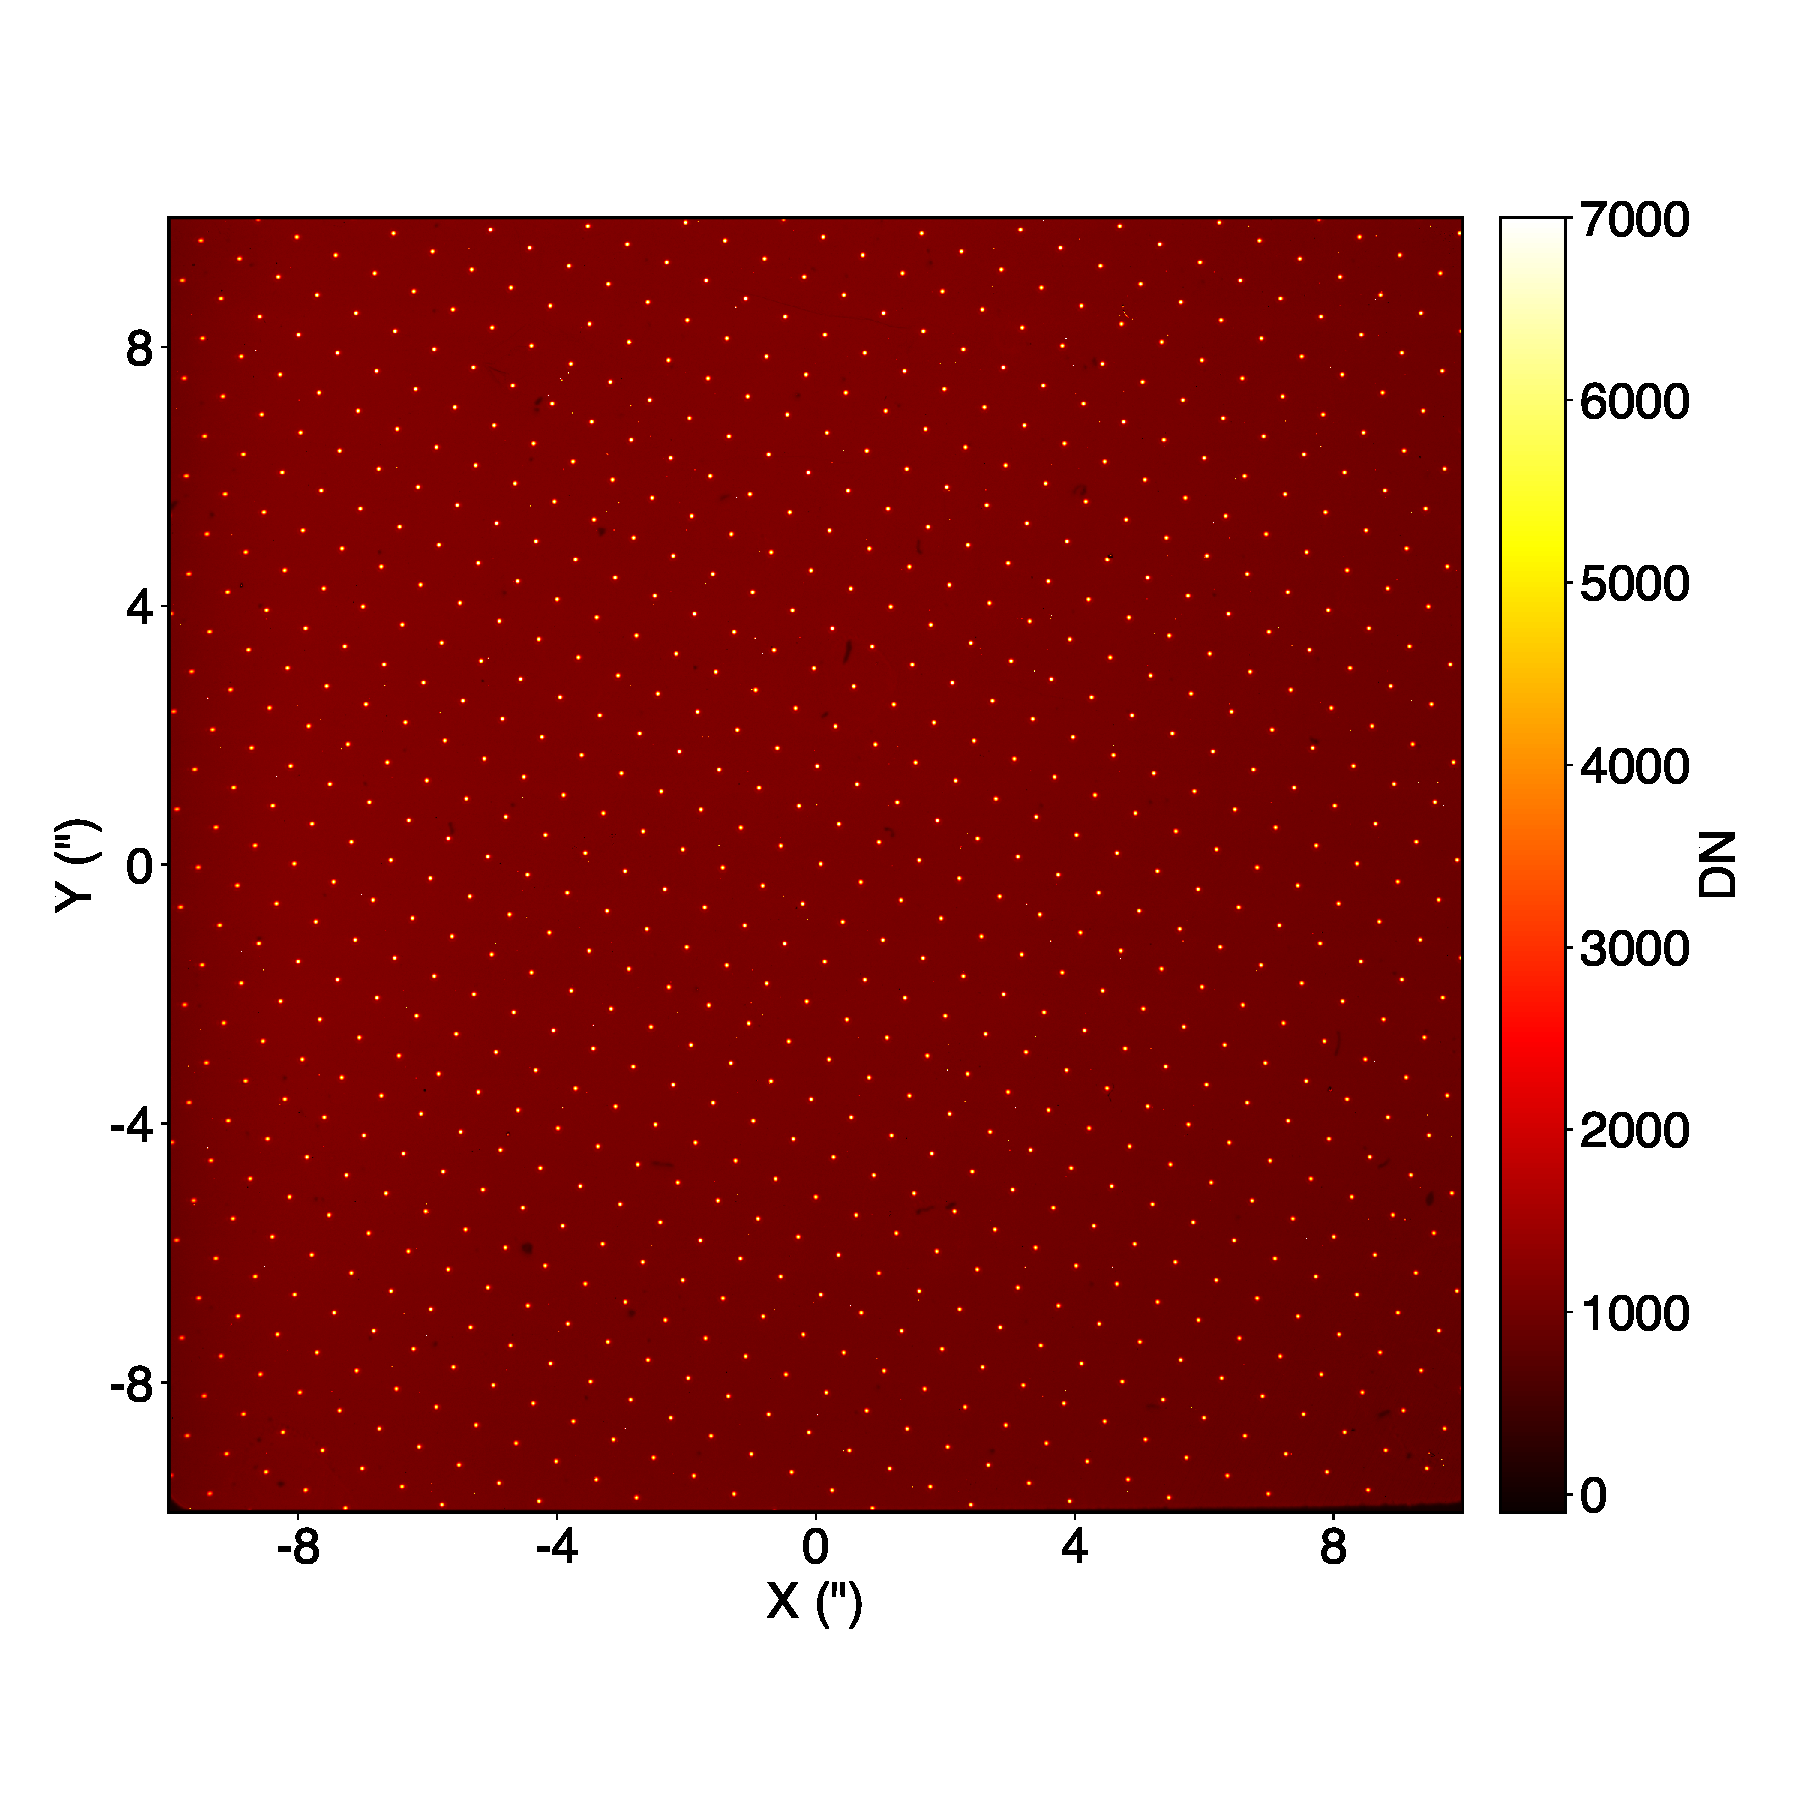
\includegraphics[width=0.8\textwidth]{airopa/Figures/osiris_pcu_grid_fullframe.pdf}
 }
 \caption{\footnotesize Full-frame image of the OSIRIS pinhole calibration unit (PCU) in focus taken in January 2023. Light from each pinhole travels through the AO system optics and OSIRIS instrument. \label{fig:pcu_grid_full}}
\end{figure}

\begin{figure}[!h]
 \makebox[\textwidth][c]{
 \hspace{-10mm}
 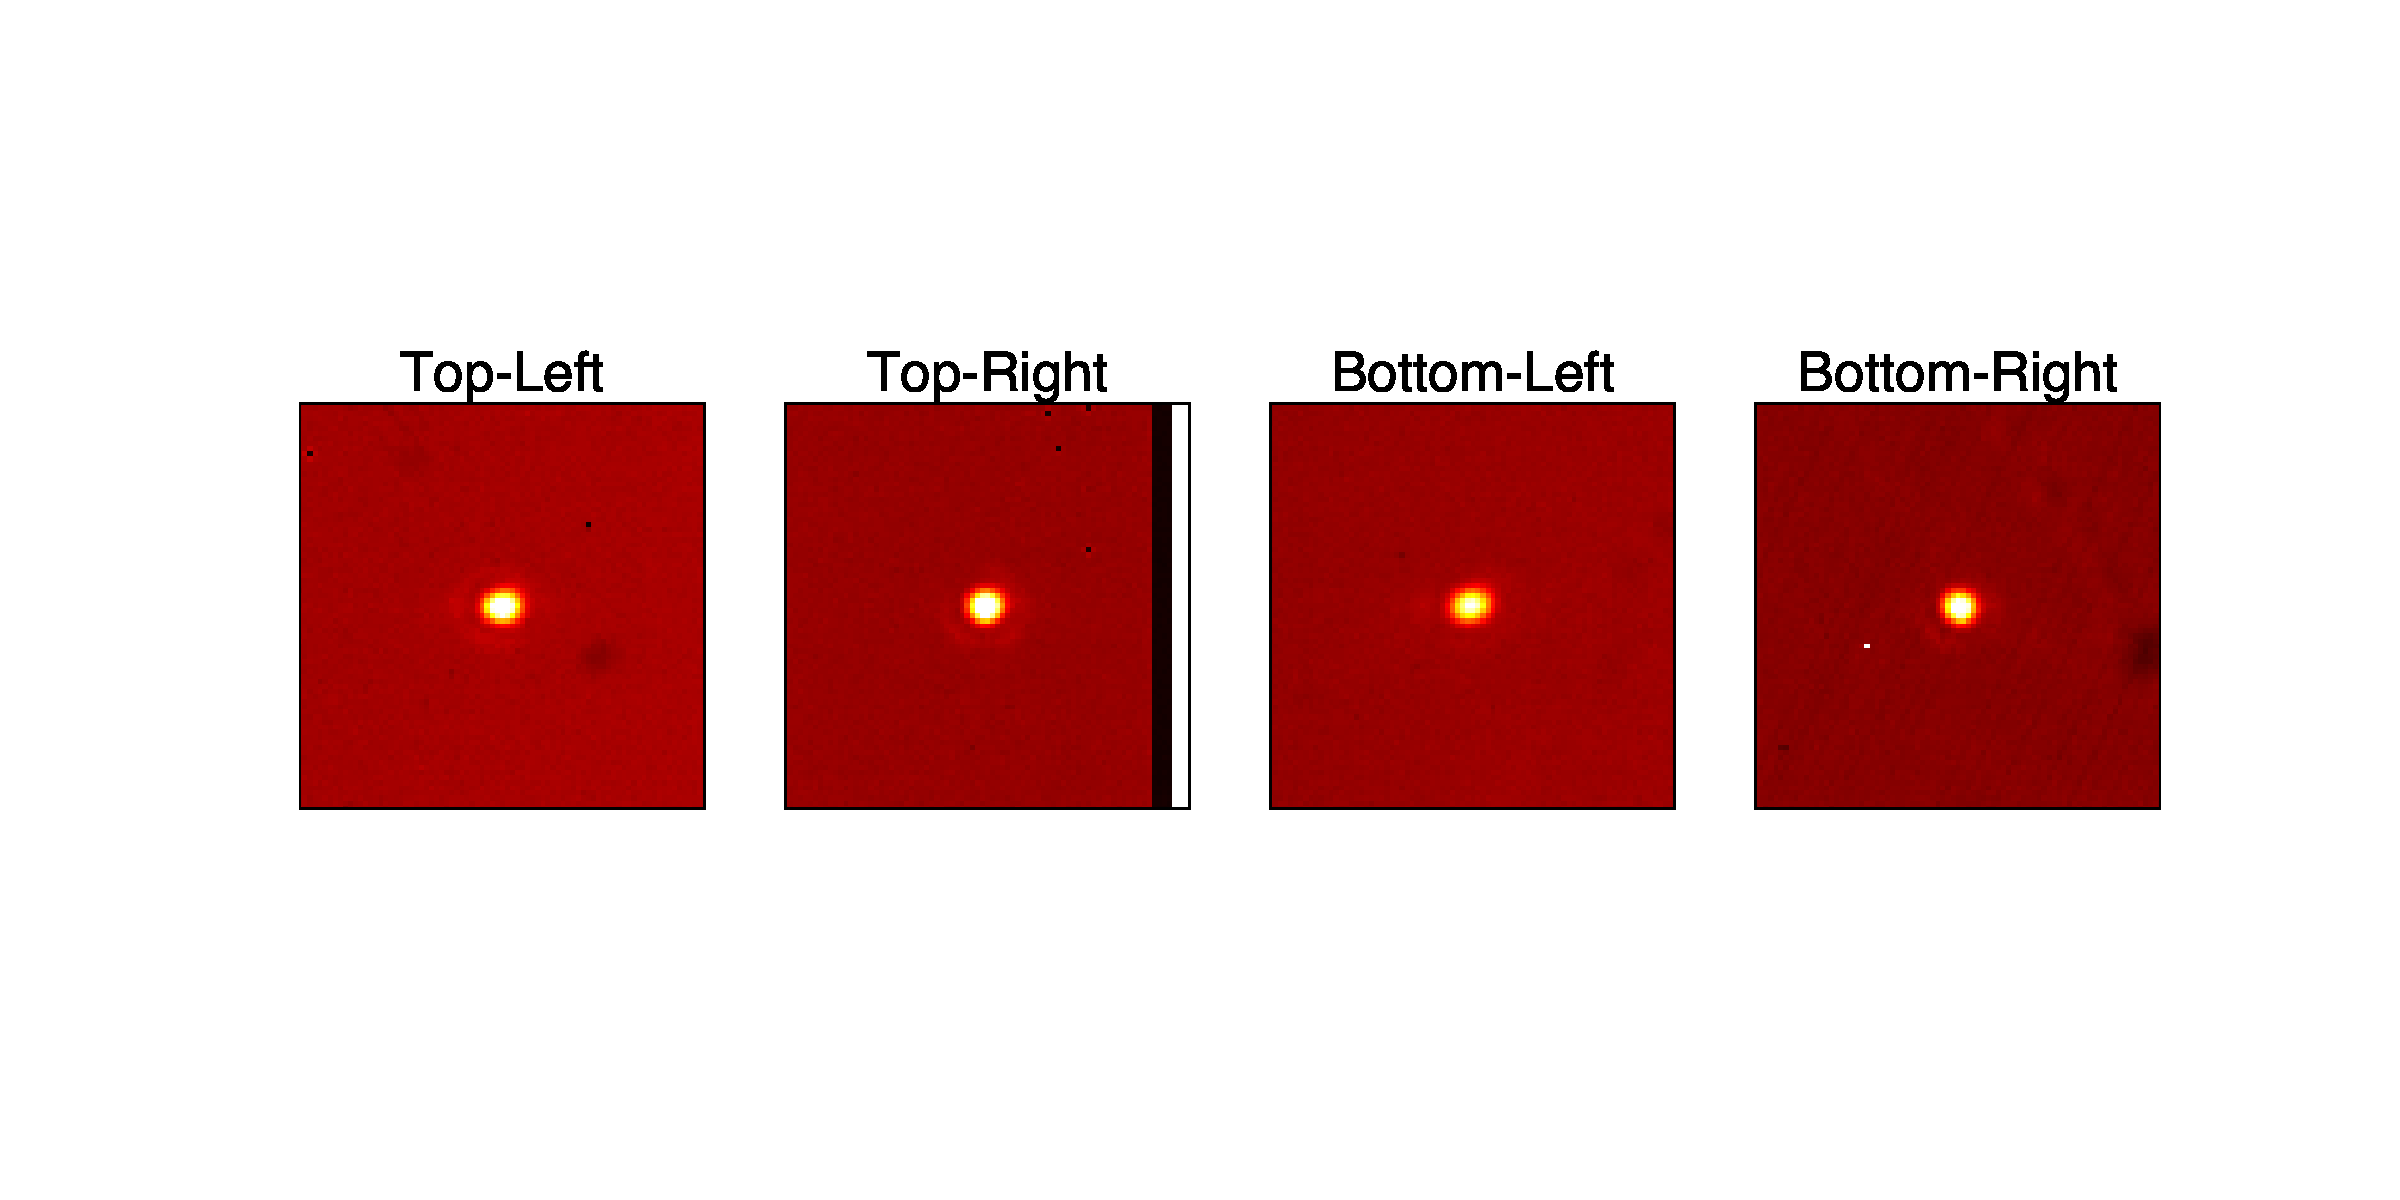
\includegraphics[width=1.2\textwidth]{airopa/Figures/osiris_pcu_grid_corners.pdf}
 }
 \vspace{-20mm}
 \caption{\footnotesize Zoomed-in view of individual pinholes shown in the four corners of Figure \ref{fig:pcu_grid_full}. The PSFs on the left-side of the field show clear elongation, while the right-side PSFs show less elongation. The color scale is the same as Figure \ref{fig:pcu_grid_full}. \label{fig:pcu_grid_corners}}
\end{figure}

\begin{figure}[!h]
 \makebox[\textwidth][c]{
 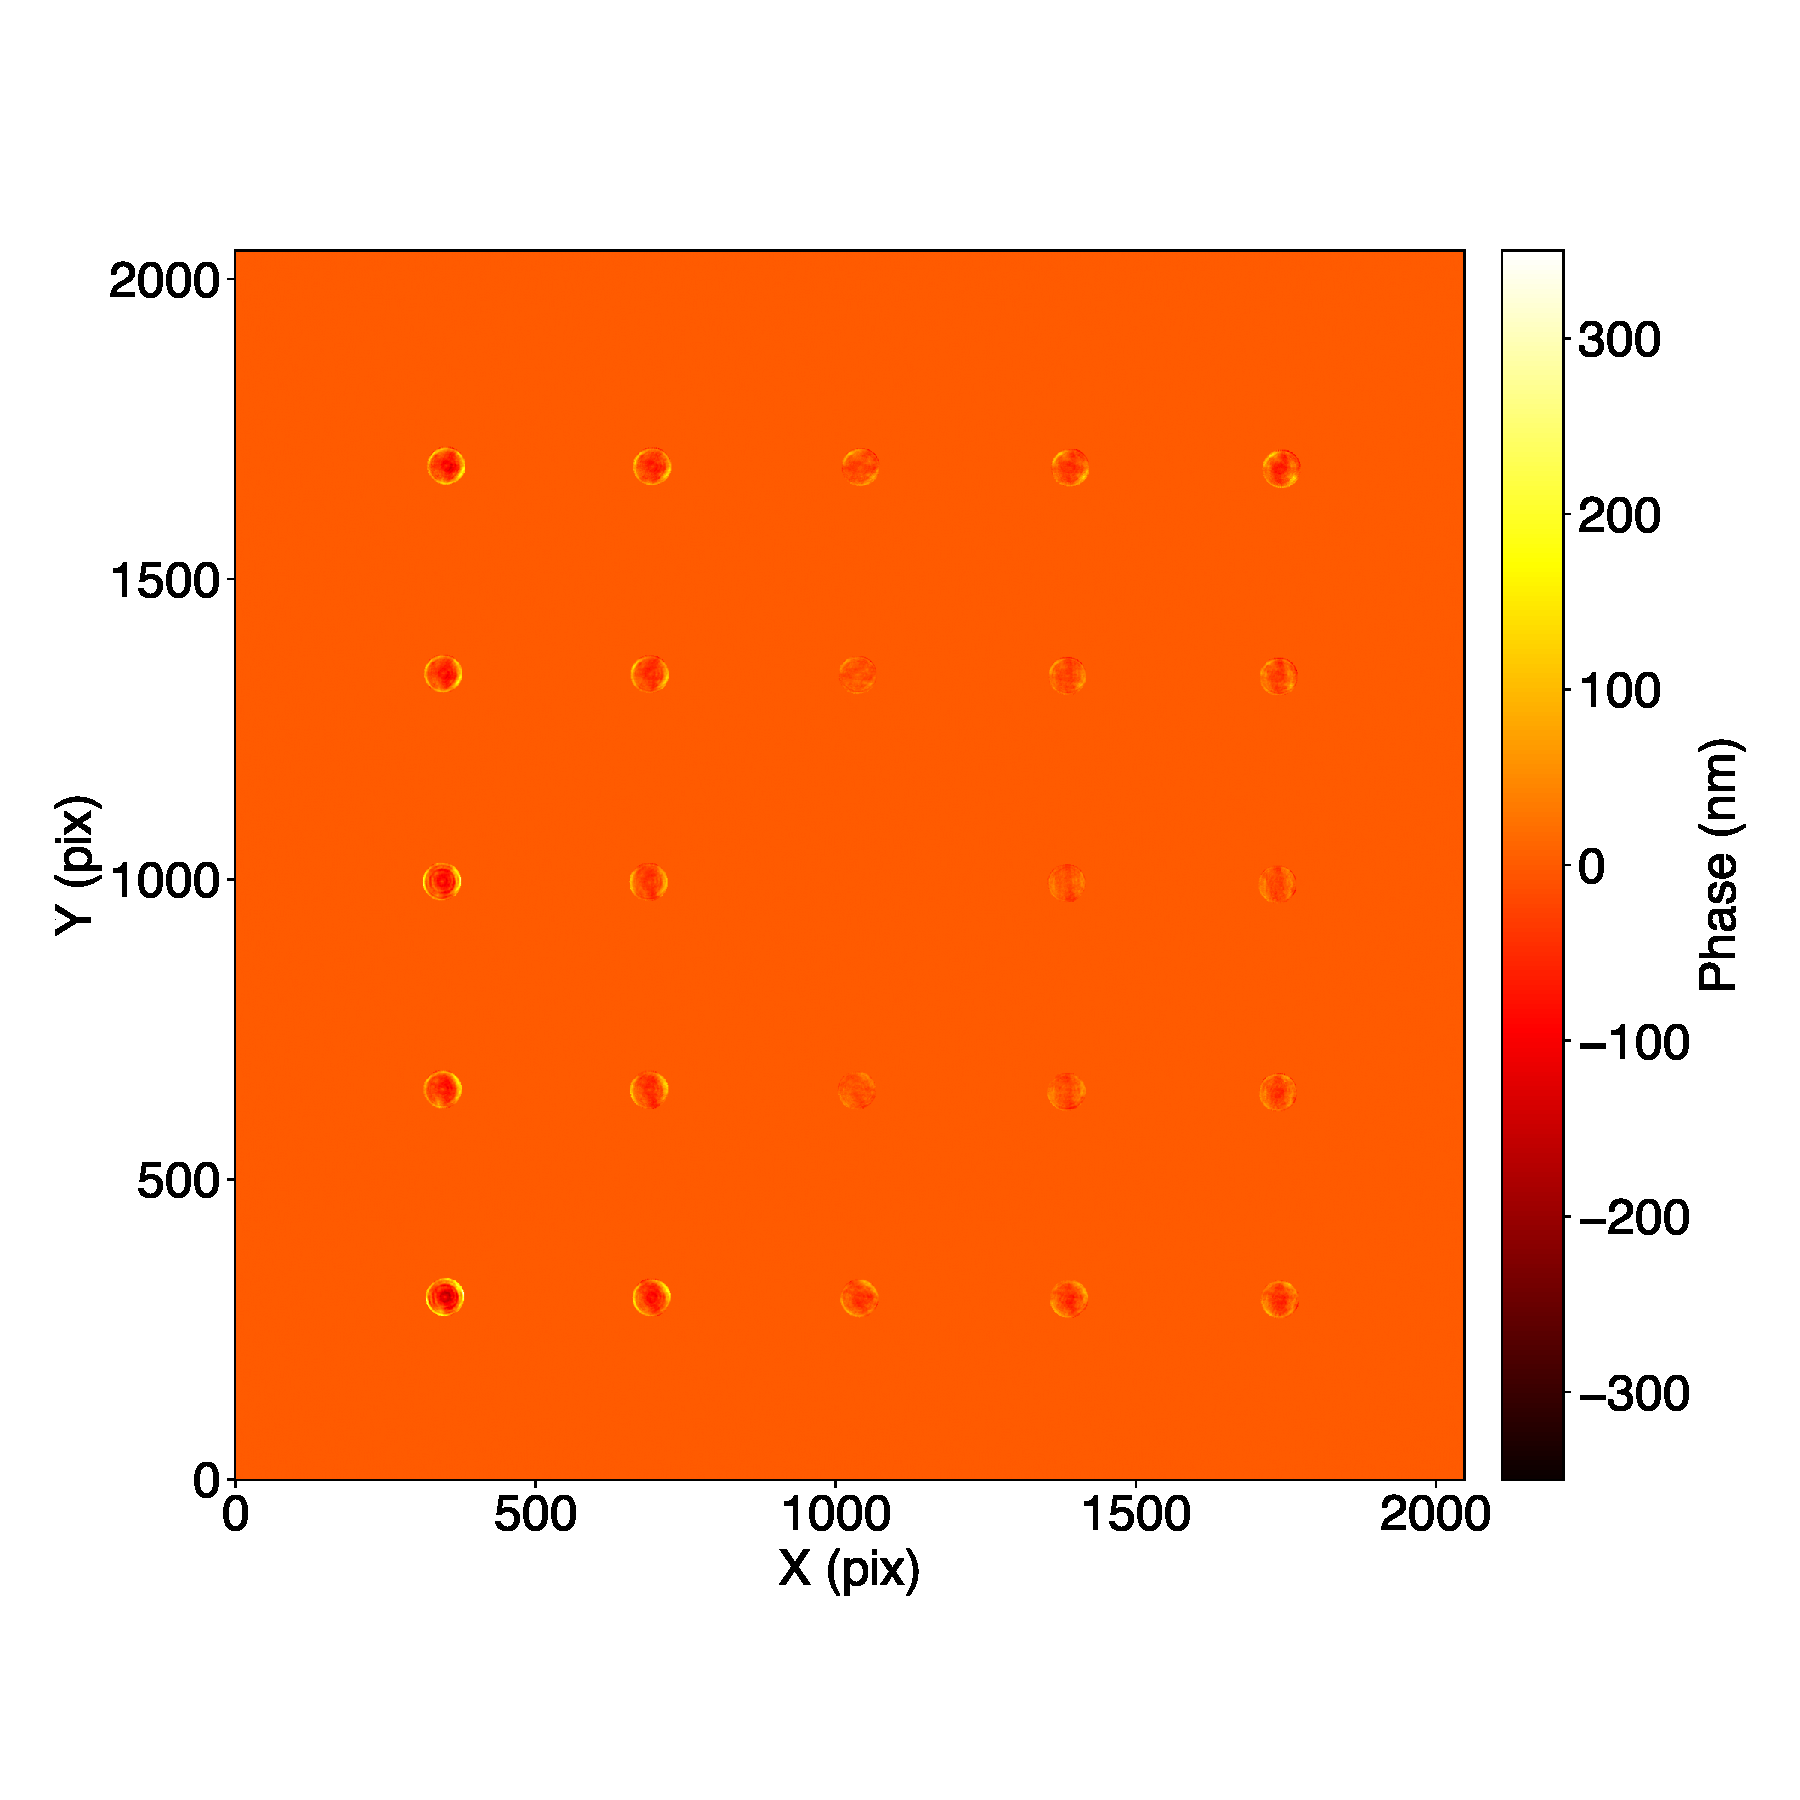
\includegraphics[width=0.9\textwidth]{airopa/Figures/osiris_phasemap_grid.pdf}
 }
 \caption{\footnotesize Center-subtracted phase map grid for the OSIRIS detector, obtained in 2020. \label{fig:phase-map-grid}}
\end{figure}

\subsection{Phase Map Retrieval} \label{subsec:phase-map-retrieval}
Describe retrieving the phase maps from the phase diversity data (Gerchberg-Saxton, etc).

\section{On-sky Observations}\label{sec:on-sky-obs}
The datasets presented in this work were acquired with the Keck-II/OSIRIS imager in the laser guide star adaptive optics (LGSAO) mode. The data were taken with the K$_{\textrm{p}}$ filter ($\lambda_{c} = 2.12\mu$m), the pixel scale for the OSIRIS imager is 9.952 mas/pix, and all of the data (including phase diversity) were taken in 2020. Figure BBB shows an individual cleaned frame from our galactic center (GC) observations with OSIRIS.

\begin{figure}[!h]
  \hspace{-20mm}
  \subfloat{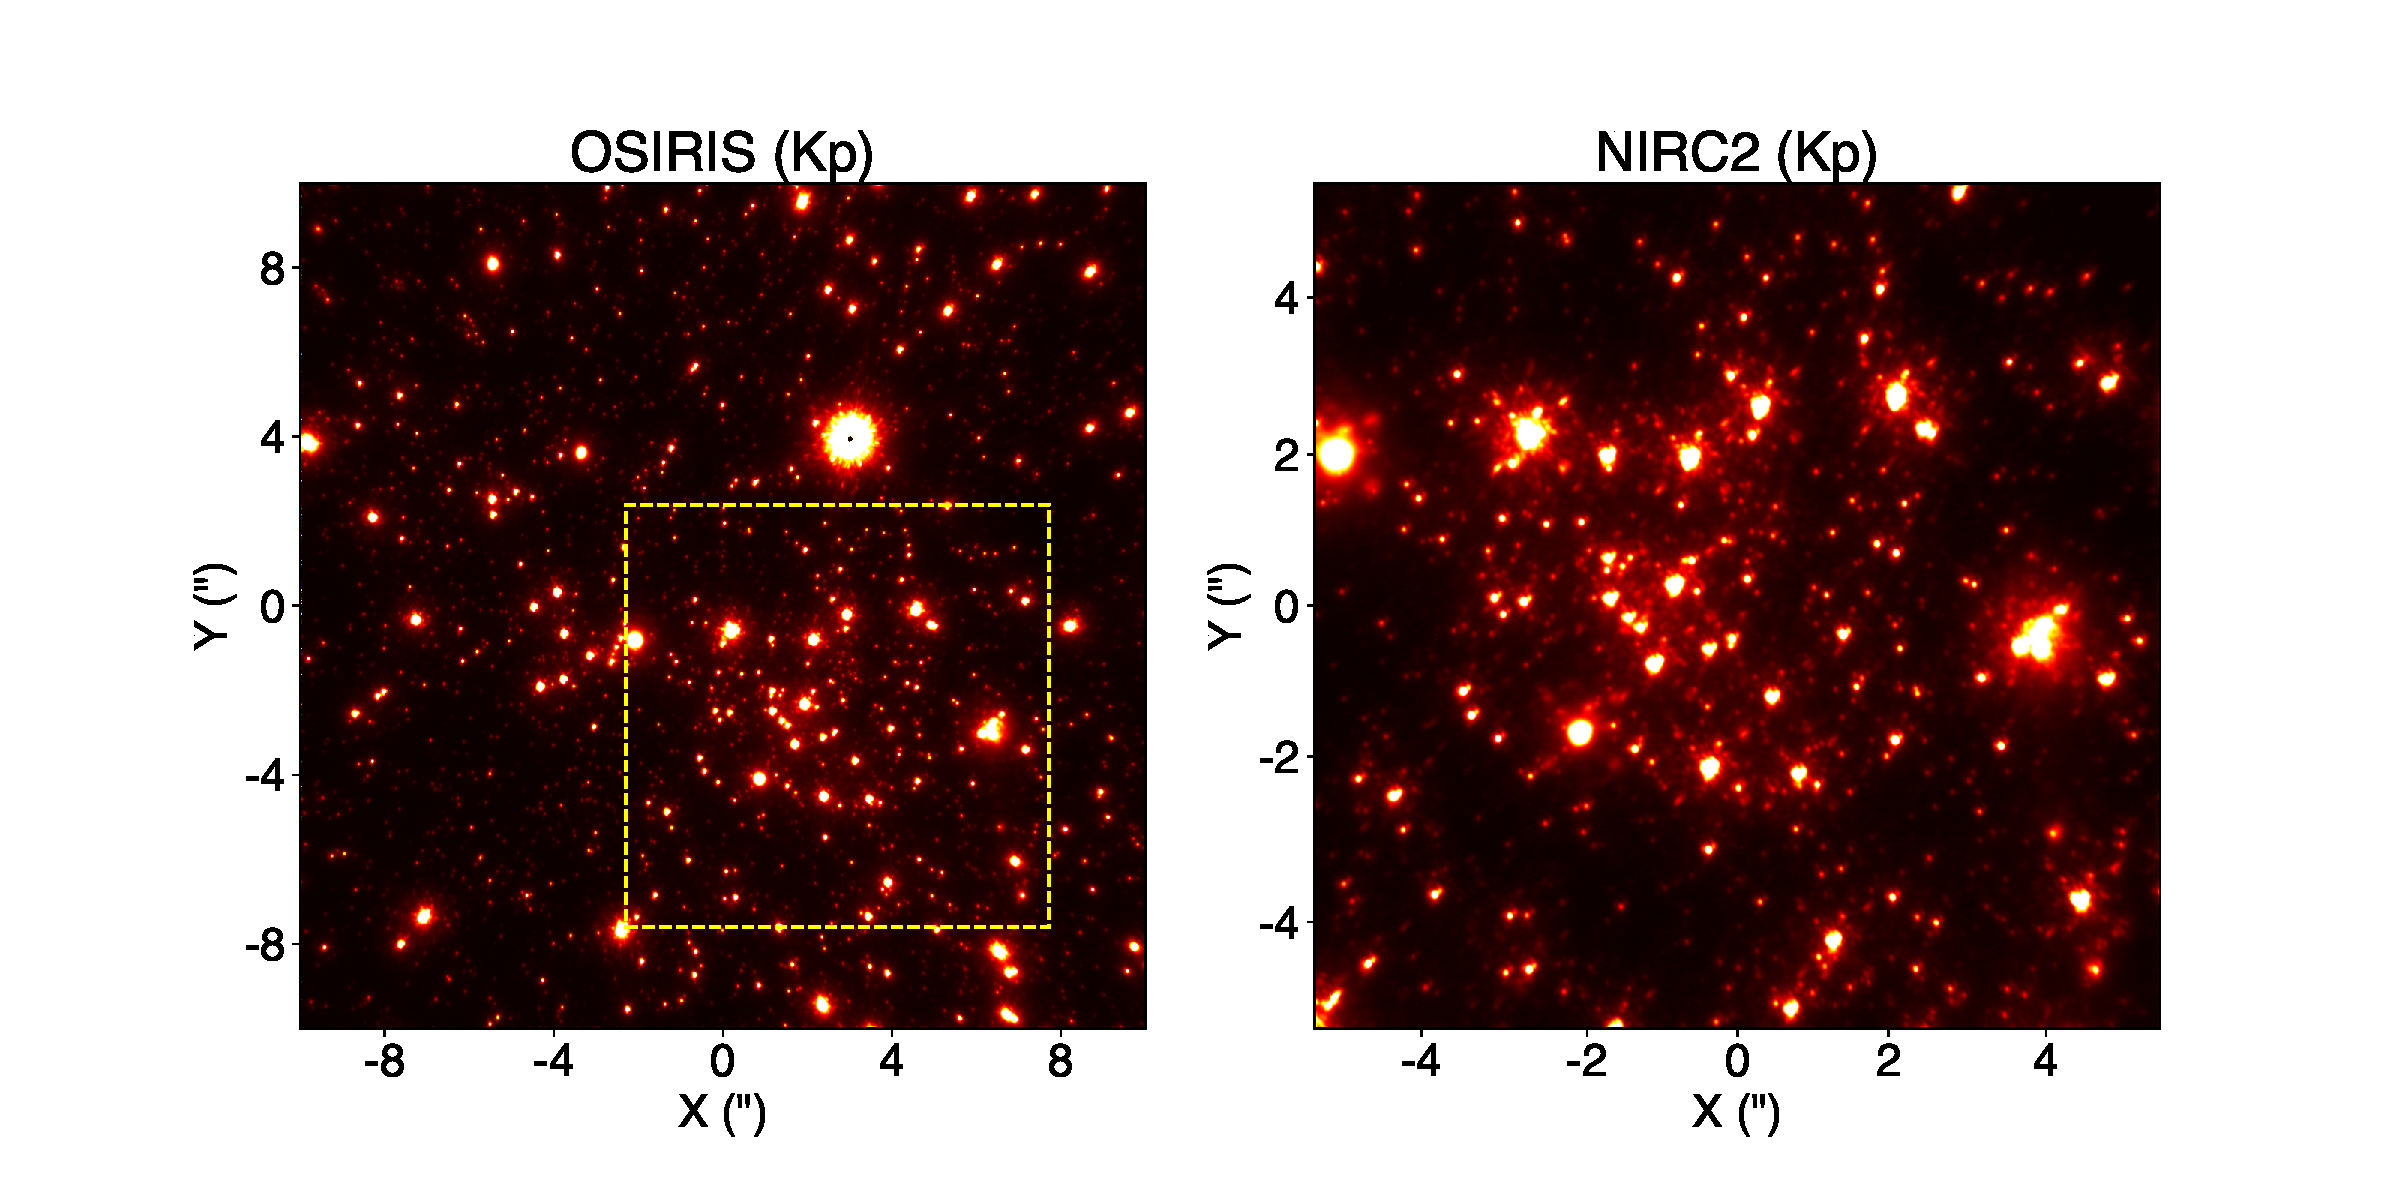
\includegraphics[width=1.2\textwidth]{airopa/Figures/gc_osiris_nirc2_image.pdf}}
  \caption{\footnotesize \textit{Left}: Full-frame OSIRIS image of the GC, with a dashed yellow outline representing the NIRC2 field of view. \textit{Right}: Full-frame NIRC2 image of the central ${\sim}10$ arcseconds around the GC.} \label{fig:gc_osiris_nirc2}
\end{figure}

% References
\bibliography{refs} % bibliography data in report.bib
\bibliographystyle{spiebib} % makes bibtex use spiebib.bst

\listoffigures

\end{document} 
